\begin{figure}[H]
\centering
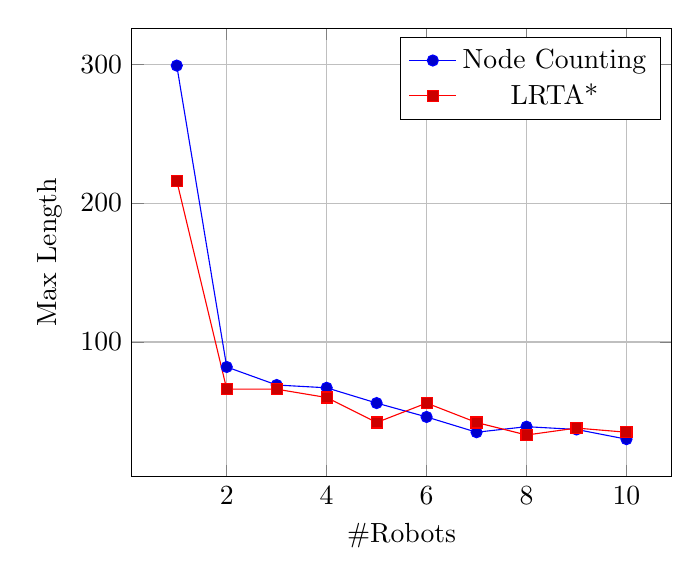
\begin{tikzpicture}
	\begin{axis}[
%		height=9cm,
%		width=9cm,
		grid=major,
		xlabel=\#Robots,
		ylabel=Max Length
	]

	\addplot coordinates {
		(1, 299)
		(2, 82)
		(3, 69)
		(4, 67)
		(5, 56)
		(6, 46)
		(7 , 35)
		(8, 39)
		(9, 37)
                (10, 30)
	};
	\addlegendentry{Node Counting}

	\addplot coordinates {
		(1, 216)
		(2, 66)
		(3, 66)
		(4, 60)
		(5, 42)
		(6, 56)
		(7 , 42)
		(8, 33)
		(9, 38)
                 (10, 35)
	};
	\addlegendentry{LRTA*}
	\end{axis}
\end{tikzpicture}
\caption{\#Robots Vs. Max Path Length}
\end{figure}


\begin{figure}[h]
\centering
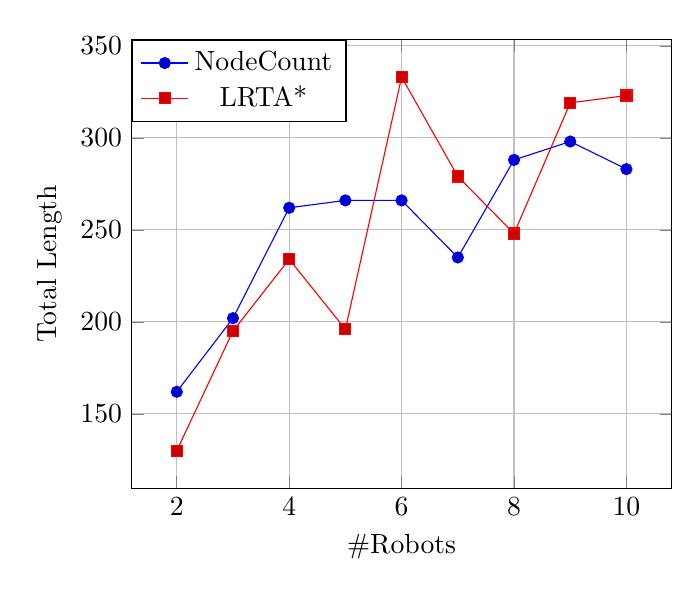
\begin{tikzpicture}
	\begin{axis}[
%		height=9cm,
%		width=9cm,
                legend style = {at={(0,1)}, anchor=north west},
		grid=major,
		xlabel=\#Robots,
		ylabel=Total Length
	]

	\addplot coordinates {
		%(1, 299)
		(2, 162)
		(3, 202)
		(4, 262)
		(5, 266)
		(6, 266)
		(7 , 235)
		(8, 288)
		(9, 298)
                (10, 283)
	};
	\addlegendentry{NodeCount}

	\addplot coordinates {
		%(1, 216)
		(2, 130)
		(3, 195)
		(4, 234)
		(5, 196)
		(6, 333)
		(7 , 279)
		(8, 248)
		(9, 319)
                 (10, 323)
	};
	\addlegendentry{LRTA*}
	\end{axis}
\end{tikzpicture}
\caption{\#Robots Vs. Total Path Length}
\end{figure}


